\documentclass[11pt,a4paper]{amsart}
\usepackage[margin=1.15in]{geometry}
\usepackage{amsmath,amssymb,amsthm}
\usepackage{tikz}
\usepackage[colorlinks=true,linkcolor=blue,citecolor=blue,urlcolor=blue]{hyperref}
\hypersetup{pdftitle={Light in a box of mirrors: counting the placements that give a single closed curve},
  pdfauthor={Cyril Shtabtsovsky},
  pdfsubject={Preprint, version 1.0, 26 November 2026. DOI 10.5281/zenodo.24546586},
  pdfkeywords={mirror curves, kolam, sona, Eulerian circuits, BEST theorem, line digraphs, Manhattan lattice, OEIS A400778}}

\newtheorem{theorem}{Theorem}
\newtheorem{corollary}[theorem]{Corollary}
\newtheorem{lemma}[theorem]{Lemma}
\newtheorem{proposition}[theorem]{Proposition}
\theoremstyle{remark}
\newtheorem{remark}[theorem]{Remark}

\newcommand{\G}{\Gamma}
\newcommand{\dout}{d^{+}}
\newcommand{\din}{d^{-}}
\newcommand{\dvv}{d_{\mathrm v}}
\newcommand{\dhh}{d_{\mathrm h}}

\title[Light in a box of mirrors]{Light in a box of mirrors:\\ counting the placements that give\\ a single closed curve}
\author[C. Shtabtsovsky]{Cyril Shtabtsovsky}
\thanks{Version 1.0. DOI: \href{https://doi.org/10.5281/zenodo.24546586}{10.5281/zenodo.24546586}. Programs: \url{https://github.com/cyrilshtabtsovsky/light-in-a-box-of-mirrors}}
\date{26 November 2026}
\subjclass[2020]{Primary 05A15; Secondary 05C45, 05C30, 05C50, 82B20}
\keywords{Mirror curves, kolam, sona, Eulerian circuits, BEST theorem, line digraphs, Manhattan lattice}

\makeatletter
\let\orig@setauthors\@setauthors
\def\@setauthors{\orig@setauthors\vskip 6pt{\centering\footnotesize\texttt{c@astrolabe.vc}\par}}
\makeatother

\begin{document}

\begin{abstract}
Place two-sided mirrors between some pairs of neighbouring dots of an $n\times k$ rectangular array of dots, and
let rays of light travel at $45^\circ$ between the dots, reflected by the mirrors and by the boundary. The rays
trace finitely many closed curves, as in the sona and kolam drawing traditions. Let $T(n,k)$ be the number of
mirror placements for which there is a single closed curve (OEIS A400778). Previously only computed values for
$n+k\le 17$ and conjectured formulas for $n\le 6$ were available. We prove the explicit product formula
\[
T(n,k)\;=\;4^{(n-1)(k-1)}\prod_{1\le l<n/2}\ \prod_{1\le m<k/2}\Bigl(1-\cos^2\frac{l\pi}{n}\,\cos^2\frac{m\pi}{k}\Bigr)
\]
for all $n$ and $k$. It implies the six conjectures stated in A400778: the formulas for $T(2,k)$ and $T(3,k)$,
the linear recurrences for $T(4,k)$, $T(5,k)$ and $T(6,k)$, and the inequality $T(n,k)\le 4^{(n-1)(k-1)}$ with
equality exactly when $\min(n,k)\le 2$. The proof starts from the observation that, once the curves are suitably
oriented, the placements counted by $T(n,k)$ are exactly the Eulerian circuits of a digraph with out-degrees at
most $2$; this holds for any finite set of dots of the square grid and expresses the count as a determinant. For
rectangular arrays
the determinant is evaluated by means of Knuth's theorem on line digraphs and an explicit diagonalisation. The
problem was chosen by the author; the formula and its proof were obtained with the AI system Claude (Anthropic,
model Fable~5.2), as described in the statement at the end of the paper.
\end{abstract}

\maketitle

\section{Introduction}

\subsection{The problem}
Take an $n\times k$ rectangular array of dots inside a box. A ray of light travels in the box at $45^\circ$ to the
walls, along the diagonal lines that pass midway between neighbouring dots, and is reflected by the walls. Between
any two neighbouring dots one may place a small two-sided mirror, which also reflects the ray. The paths of all
such rays form finitely many closed curves, the \emph{mirror curve} of the placement, and every dot is enclosed by
them (Figure~\ref{fig:examples}).

\begin{figure}[ht]
\centering
\begin{tabular}{ccc}
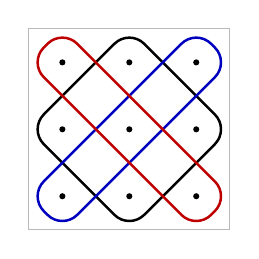
\begin{tikzpicture}[scale=0.85,line cap=round]
\draw[gray!55,thin] (0,0) rectangle (3,3);
\draw[black,line width=0.9pt,rounded corners=7.6pt] (0.5,1.0) -- (1.0,0.5) -- (1.5,0.0) -- (2.0,0.5) -- (2.5,1.0) -- (3.0,1.5) -- (2.5,2.0) -- (2.0,2.5) -- (1.5,3.0) -- (1.0,2.5) -- (0.5,2.0) -- (0.0,1.5) -- cycle;
\draw[blue!75!black,line width=0.9pt,rounded corners=7.6pt] (1.0,0.5) -- (0.5,0.0) -- (0.0,0.5) -- (0.5,1.0) -- (1.0,1.5) -- (1.5,2.0) -- (2.0,2.5) -- (2.5,3.0) -- (3.0,2.5) -- (2.5,2.0) -- (2.0,1.5) -- (1.5,1.0) -- cycle;
\draw[red!75!black,line width=0.9pt,rounded corners=7.6pt] (1.0,1.5) -- (0.5,2.0) -- (0.0,2.5) -- (0.5,3.0) -- (1.0,2.5) -- (1.5,2.0) -- (2.0,1.5) -- (2.5,1.0) -- (3.0,0.5) -- (2.5,0.0) -- (2.0,0.5) -- (1.5,1.0) -- cycle;
\fill (0.5,0.5) circle (1.3pt);
\fill (0.5,1.5) circle (1.3pt);
\fill (0.5,2.5) circle (1.3pt);
\fill (1.5,0.5) circle (1.3pt);
\fill (1.5,1.5) circle (1.3pt);
\fill (1.5,2.5) circle (1.3pt);
\fill (2.5,0.5) circle (1.3pt);
\fill (2.5,1.5) circle (1.3pt);
\fill (2.5,2.5) circle (1.3pt);
\end{tikzpicture} & 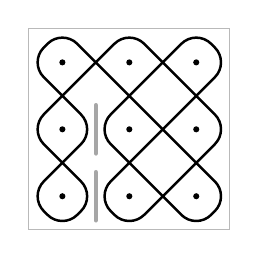
\begin{tikzpicture}[scale=0.85,line cap=round]
\draw[gray!55,thin] (0,0) rectangle (3,3);
\draw[line width=1.6pt,gray!70] (1,0.14) -- (1,0.86);
\draw[line width=1.6pt,gray!70] (1,1.14) -- (1,1.86);
\draw[black,line width=0.9pt,rounded corners=7.6pt] (0.5,1.0) -- (1.0,0.5) -- (0.5,0.0) -- (0.0,0.5) -- (0.5,1.0) -- (1.0,1.5) -- (0.5,2.0) -- (0.0,2.5) -- (0.5,3.0) -- (1.0,2.5) -- (1.5,2.0) -- (2.0,1.5) -- (2.5,1.0) -- (3.0,0.5) -- (2.5,0.0) -- (2.0,0.5) -- (1.5,1.0) -- (1.0,1.5) -- (1.5,2.0) -- (2.0,2.5) -- (2.5,3.0) -- (3.0,2.5) -- (2.5,2.0) -- (2.0,1.5) -- (1.5,1.0) -- (1.0,0.5) -- (1.5,0.0) -- (2.0,0.5) -- (2.5,1.0) -- (3.0,1.5) -- (2.5,2.0) -- (2.0,2.5) -- (1.5,3.0) -- (1.0,2.5) -- (0.5,2.0) -- (0.0,1.5) -- cycle;
\fill (0.5,0.5) circle (1.3pt);
\fill (0.5,1.5) circle (1.3pt);
\fill (0.5,2.5) circle (1.3pt);
\fill (1.5,0.5) circle (1.3pt);
\fill (1.5,1.5) circle (1.3pt);
\fill (1.5,2.5) circle (1.3pt);
\fill (2.5,0.5) circle (1.3pt);
\fill (2.5,1.5) circle (1.3pt);
\fill (2.5,2.5) circle (1.3pt);
\end{tikzpicture} & 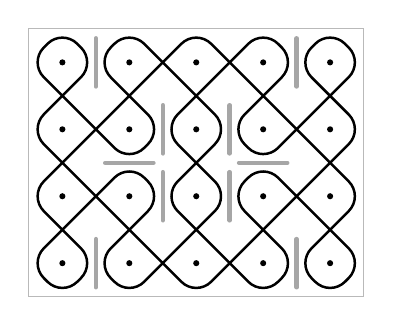
\begin{tikzpicture}[scale=0.85,line cap=round]
\draw[gray!55,thin] (0,0) rectangle (5,4);
\draw[line width=1.6pt,gray!70] (2,1.14) -- (2,1.86);
\draw[line width=1.6pt,gray!70] (3.14,2) -- (3.86,2);
\draw[line width=1.6pt,gray!70] (1,0.14) -- (1,0.86);
\draw[line width=1.6pt,gray!70] (1,3.14) -- (1,3.86);
\draw[line width=1.6pt,gray!70] (4,0.14) -- (4,0.86);
\draw[line width=1.6pt,gray!70] (1.14,2) -- (1.86,2);
\draw[line width=1.6pt,gray!70] (2,2.14) -- (2,2.86);
\draw[line width=1.6pt,gray!70] (3,2.14) -- (3,2.86);
\draw[line width=1.6pt,gray!70] (4,3.14) -- (4,3.86);
\draw[line width=1.6pt,gray!70] (3,1.14) -- (3,1.86);
\draw[black,line width=0.9pt,rounded corners=7.6pt] (0.5,1.0) -- (1.0,0.5) -- (0.5,0.0) -- (0.0,0.5) -- (0.5,1.0) -- (1.0,1.5) -- (1.5,2.0) -- (2.0,1.5) -- (1.5,1.0) -- (1.0,0.5) -- (1.5,0.0) -- (2.0,0.5) -- (2.5,1.0) -- (3.0,1.5) -- (2.5,2.0) -- (2.0,2.5) -- (2.5,3.0) -- (3.0,3.5) -- (3.5,4.0) -- (4.0,3.5) -- (3.5,3.0) -- (3.0,2.5) -- (3.5,2.0) -- (4.0,2.5) -- (4.5,3.0) -- (5.0,3.5) -- (4.5,4.0) -- (4.0,3.5) -- (4.5,3.0) -- (5.0,2.5) -- (4.5,2.0) -- (4.0,1.5) -- (3.5,1.0) -- (3.0,0.5) -- (2.5,0.0) -- (2.0,0.5) -- (1.5,1.0) -- (1.0,1.5) -- (0.5,2.0) -- (0.0,2.5) -- (0.5,3.0) -- (1.0,3.5) -- (0.5,4.0) -- (0.0,3.5) -- (0.5,3.0) -- (1.0,2.5) -- (1.5,2.0) -- (2.0,2.5) -- (1.5,3.0) -- (1.0,3.5) -- (1.5,4.0) -- (2.0,3.5) -- (2.5,3.0) -- (3.0,2.5) -- (2.5,2.0) -- (2.0,1.5) -- (2.5,1.0) -- (3.0,0.5) -- (3.5,0.0) -- (4.0,0.5) -- (3.5,1.0) -- (3.0,1.5) -- (3.5,2.0) -- (4.0,1.5) -- (4.5,1.0) -- (5.0,0.5) -- (4.5,0.0) -- (4.0,0.5) -- (4.5,1.0) -- (5.0,1.5) -- (4.5,2.0) -- (4.0,2.5) -- (3.5,3.0) -- (3.0,3.5) -- (2.5,4.0) -- (2.0,3.5) -- (1.5,3.0) -- (1.0,2.5) -- (0.5,2.0) -- (0.0,1.5) -- cycle;
\fill (0.5,0.5) circle (1.3pt);
\fill (0.5,1.5) circle (1.3pt);
\fill (0.5,2.5) circle (1.3pt);
\fill (0.5,3.5) circle (1.3pt);
\fill (1.5,0.5) circle (1.3pt);
\fill (1.5,1.5) circle (1.3pt);
\fill (1.5,2.5) circle (1.3pt);
\fill (1.5,3.5) circle (1.3pt);
\fill (2.5,0.5) circle (1.3pt);
\fill (2.5,1.5) circle (1.3pt);
\fill (2.5,2.5) circle (1.3pt);
\fill (2.5,3.5) circle (1.3pt);
\fill (3.5,0.5) circle (1.3pt);
\fill (3.5,1.5) circle (1.3pt);
\fill (3.5,2.5) circle (1.3pt);
\fill (3.5,3.5) circle (1.3pt);
\fill (4.5,0.5) circle (1.3pt);
\fill (4.5,1.5) circle (1.3pt);
\fill (4.5,2.5) circle (1.3pt);
\fill (4.5,3.5) circle (1.3pt);
\end{tikzpicture}\\[2pt]
(a) & (b) & (c)
\end{tabular}
\caption{Mirror curves. Mirrors are drawn as grey bars. (a) The $3\times3$ array without mirrors: three curves.
(b) Two mirrors: one curve. (c) A $5\times4$ array with ten mirrors: one curve.}\label{fig:examples}
\end{figure}

Without mirrors the number of curves is $\gcd(n,k)$ \cite{FM,Gerdes,JRSZ}; mirrors merge and split curves. There
are $M=2nk-n-k$ positions for a mirror, hence $2^{M}$ placements. This paper answers the question:
\emph{for how many placements is the mirror curve a single closed curve?} We denote this number by $T(n,k)$. For
example $T(3,3)=240$, out of $2^{12}=4096$ placements.

\subsection{Background}
Mirror curves were introduced by Gerdes \cite{Gerdes} to describe the \emph{sona}, drawings traced in the sand by
the Chokwe people of Angola. The same curves describe the \emph{kolam} drawings of South India
\cite{Ishimoto,Nagata,YN} and the plaitwork panels of Celtic art \cite{FM,JRSZ}. In the sona and kolam traditions a drawing that consists of one closed line, and can therefore be
traced without lifting the finger, has a special status; such drawings are called monolinear, one-stroke, or
infinite \cite{Gerdes,Ishimoto,YN}. If the points where the curve crosses itself are read as crossings of a knot
diagram, a mirror curve is a link and a single curve is a knot \cite{JRSZ}.

The number of curves of a given placement can be computed from the Tutte polynomial of an associated graph
\cite{Nagata}. The number of placements with a single curve has been determined before only by exhaustive computer
search. For the diamond-shaped array with rows of $1,3,5,3,1$ dots, Yanagisawa and Nagata \cite{YN} found $240$
single-curve placements among $2^{16}$, and for the array with rows of $1,3,5,7,5,3,1$ dots they found
$11\,661\,312$ among $2^{36}$ (the ``1-5-1'' and ``1-7-1'' arrays of \cite{YN}); see also \cite{Ishimoto}. For rectangular arrays the values of $T(n,k)$ with
$n+k\le 17$ are listed in the OEIS \cite{OEIS}, together with six conjectured formulas.

\subsection{Result}
The main result (Theorem~\ref{thm:main}) is the product formula
\[
T(n,k)\;=\;4^{(n-1)(k-1)}\prod_{1\le l<n/2}\ \prod_{1\le m<k/2}\Bigl(1-\cos^2\frac{l\pi}{n}\,\cos^2\frac{m\pi}{k}\Bigr)
\]
for all $n$ and $k$. The six conjectures of \cite{OEIS} follow from it
(Corollaries~\ref{cor:rows} and~\ref{cor:ineq}). To our knowledge the following are new:
\begin{enumerate}
\item[(i)] the observation that, after a suitable orientation of the curve, the placements with a single curve are
the Eulerian circuits of a digraph in which every vertex has out-degree at most $2$, so that their number is a
determinant; this holds for every finite set of dots of the square grid (Remark~\ref{rem:shapes});
\item[(ii)] the product formula for rectangular arrays;
\item[(iii)] the proofs of the formulas conjectured in \cite{OEIS}.
\end{enumerate}

\subsection{Related formulas}
The formula for $T(n,k)$ is of the same type as two classical formulas for rectangular pieces of the square
lattice (Figure~\ref{fig:relatives}). The number of domino tilings of an $m\times n$ board is
\cite{Kasteleyn61,TF}
\[ \prod_{j=1}^{\lceil m/2\rceil}\ \prod_{l=1}^{\lceil n/2\rceil}\Bigl(4\cos^2\frac{j\pi}{m+1}+4\cos^2\frac{l\pi}{n+1}\Bigr), \]
and the number of spanning trees of the $m\times n$ grid graph is (see \cite{KPW})
\[ \frac{1}{mn}\prod_{\substack{0\le j<m,\ 0\le l<n\\ (j,l)\ne(0,0)}}\Bigl(4-2\cos\frac{j\pi}{m}-2\cos\frac{l\pi}{n}\Bigr). \]
The relation with spanning trees is exact: $T(n,k)^2$ is $4^{(n-1)(k-1)}$ times the number of spanning trees of a
graph on the corners of the array (Remark~\ref{rem:trees}). The exponential growth rates of all three counts
involve Catalan's constant (Corollary~\ref{cor:growth}). The digraph in (i) is a piece of the Manhattan lattice,
on which Kasteleyn \cite{Kasteleyn} counted Hamiltonian walks by a related argument; see also \cite{DD} and
Remark~\ref{rem:manhattan}.

\begin{figure}[ht]
\centering
\begin{tabular}{ccc}
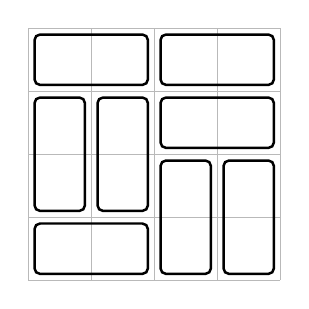
\begin{tikzpicture}[scale=0.8]
\draw[gray!55,thin] (0,0) grid (4,4);
\foreach \x/\y/\w/\h in {0/0/2/1, 2/0/1/2, 3/0/1/2, 0/1/1/2, 1/1/1/2, 2/2/2/1, 0/3/2/1, 2/3/2/1}{
  \draw[line width=0.9pt,rounded corners=2pt] (\x+0.1,\y+0.1) rectangle (\x+\w-0.1,\y+\h-0.1);}
\end{tikzpicture} & 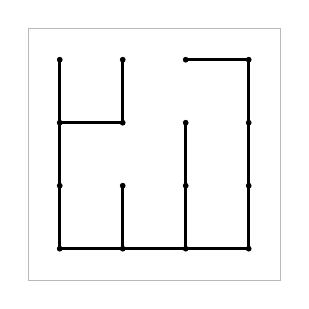
\begin{tikzpicture}[scale=0.8]
\draw[gray!55,thin] (0,0) rectangle (4,4);
\draw[line width=0.9pt] (0.5,0.5)--(3.5,0.5) (0.5,0.5)--(0.5,3.5) (1.5,0.5)--(1.5,1.5) (2.5,0.5)--(2.5,2.5) (3.5,0.5)--(3.5,3.5) (0.5,2.5)--(1.5,2.5) (1.5,2.5)--(1.5,3.5) (2.5,3.5)--(3.5,3.5);
\foreach \i in {1,...,4}{\foreach \j in {1,...,4}{\fill (\i-0.5,\j-0.5) circle (1.3pt);}}
\end{tikzpicture} & 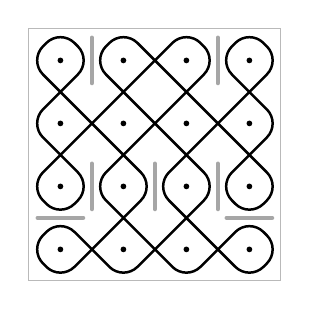
\begin{tikzpicture}[scale=0.8,line cap=round]
\draw[gray!55,thin] (0,0) rectangle (4,4);
\draw[line width=1.6pt,gray!70] (1,3.14) -- (1,3.86);
\draw[line width=1.6pt,gray!70] (2,1.14) -- (2,1.86);
\draw[line width=1.6pt,gray!70] (3,3.14) -- (3,3.86);
\draw[line width=1.6pt,gray!70] (1,1.14) -- (1,1.86);
\draw[line width=1.6pt,gray!70] (3.14,1) -- (3.86,1);
\draw[line width=1.6pt,gray!70] (0.14,1) -- (0.86,1);
\draw[line width=1.6pt,gray!70] (3,1.14) -- (3,1.86);
\draw[black,line width=0.9pt,rounded corners=7.2pt] (0.5,1.0) -- (1.0,0.5) -- (1.5,0.0) -- (2.0,0.5) -- (2.5,1.0) -- (3.0,1.5) -- (2.5,2.0) -- (2.0,2.5) -- (1.5,3.0) -- (1.0,3.5) -- (1.5,4.0) -- (2.0,3.5) -- (2.5,3.0) -- (3.0,2.5) -- (3.5,2.0) -- (4.0,1.5) -- (3.5,1.0) -- (3.0,1.5) -- (3.5,2.0) -- (4.0,2.5) -- (3.5,3.0) -- (3.0,3.5) -- (3.5,4.0) -- (4.0,3.5) -- (3.5,3.0) -- (3.0,2.5) -- (2.5,2.0) -- (2.0,1.5) -- (2.5,1.0) -- (3.0,0.5) -- (3.5,0.0) -- (4.0,0.5) -- (3.5,1.0) -- (3.0,0.5) -- (2.5,0.0) -- (2.0,0.5) -- (1.5,1.0) -- (1.0,1.5) -- (1.5,2.0) -- (2.0,2.5) -- (2.5,3.0) -- (3.0,3.5) -- (2.5,4.0) -- (2.0,3.5) -- (1.5,3.0) -- (1.0,2.5) -- (0.5,2.0) -- (0.0,1.5) -- (0.5,1.0) -- (1.0,1.5) -- (0.5,2.0) -- (0.0,2.5) -- (0.5,3.0) -- (1.0,3.5) -- (0.5,4.0) -- (0.0,3.5) -- (0.5,3.0) -- (1.0,2.5) -- (1.5,2.0) -- (2.0,1.5) -- (1.5,1.0) -- (1.0,0.5) -- (0.5,0.0) -- (0.0,0.5) -- cycle;
\fill (0.5,0.5) circle (1.3pt);
\fill (0.5,1.5) circle (1.3pt);
\fill (0.5,2.5) circle (1.3pt);
\fill (0.5,3.5) circle (1.3pt);
\fill (1.5,0.5) circle (1.3pt);
\fill (1.5,1.5) circle (1.3pt);
\fill (1.5,2.5) circle (1.3pt);
\fill (1.5,3.5) circle (1.3pt);
\fill (2.5,0.5) circle (1.3pt);
\fill (2.5,1.5) circle (1.3pt);
\fill (2.5,2.5) circle (1.3pt);
\fill (2.5,3.5) circle (1.3pt);
\fill (3.5,0.5) circle (1.3pt);
\fill (3.5,1.5) circle (1.3pt);
\fill (3.5,2.5) circle (1.3pt);
\fill (3.5,3.5) circle (1.3pt);
\end{tikzpicture}\\[2pt]
(a) & (b) & (c)
\end{tabular}
\caption{Three objects on a $4\times4$ grid whose numbers are given by double cosine products: (a) a domino
tiling, (b) a spanning tree, (c) a mirror placement with a single curve.}\label{fig:relatives}
\end{figure}

\section{Definitions and results}

\subsection{Definitions}
Fix integers $n,k\ge 1$. The \emph{cells} are the unit squares $Q_{ij}=[i-1,i]\times[j-1,j]$, $1\le i\le n$,
$1\le j\le k$; each has a dot at its centre. The \emph{corners} are the lattice points $(p,q)$ with $0\le p\le n$,
$0\le q\le k$, and the \emph{sides} are the unit segments joining adjacent corners. There are $2nk+n+k$ sides; the
$2n+2k$ sides on the boundary of the rectangle are \emph{border sides} and the remaining
\[ M=2nk-n-k \]
sides, each shared by two cells, are \emph{internal sides}. A \emph{mirror placement} is a set $X$ of internal
sides.

In each cell draw the four segments joining the midpoints of adjacent sides; we call them \emph{arcs}. The arcs
of a cell form a diamond around its dot. Given $X$, glue arcs at the midpoint $P$ of each side $s$ as follows.
\begin{itemize}
\item If $s$ is a border side or $s\in X$ (the ray is reflected), the two arcs of each cell that end at $P$ are
glued to each other.
\item If $s$ is internal and $s\notin X$ (the ray passes straight through), each arc ending at $P$ is glued to
the collinear arc in the other cell.
\end{itemize}
The arcs then form a finite set of closed polygons, the \emph{mirror curve} of $X$; see
\cite{Gerdes,JRSZ}. Let $T(n,k)$ be the number of the $2^{M}$ mirror placements whose mirror curve is a single
closed polygon. This is the array A400778 of \cite{OEIS}, where its symmetry $T(n,k)=T(k,n)$ and $T(1,k)=1$ are noted
and six formulas are stated as conjectures on the basis of computed values.

\subsection{Results}
Throughout, $g=(n-1)(k-1)$ is the number of corners in the interior of the rectangle.

\begin{theorem}\label{thm:main}
For all $n,k\ge 1$,
\begin{align}
T(n,k)&=4^{(n-1)(k-1)}\prod_{l=1}^{n-1}\prod_{m=1}^{k-1}\Bigl(1-\cos\frac{l\pi}{n}\cos\frac{m\pi}{k}\Bigr)^{1/2}
\label{eq:main}\\
&=4^{(n-1)(k-1)}\prod_{1\le l<n/2}\ \prod_{1\le m<k/2}\Bigl(1-\cos^2\frac{l\pi}{n}\cos^2\frac{m\pi}{k}\Bigr).
\label{eq:main2}
\end{align}
Equivalently, $T(n,k)^2=\det\bigl(16\,I-4\,A_{n-1}\otimes A_{k-1}\bigr)$, where $A_r$ is the adjacency matrix of the
path with $r$ vertices.
\end{theorem}

The two products agree because the four index pairs $(l,m)$, $(n-l,m)$, $(l,k-m)$, $(n-l,k-m)$ contribute
$(1-c)^2(1+c)^2$ with $c=\cos\frac{l\pi}n\cos\frac{m\pi}k$, and $c=0$ if $l=n/2$ or $m=k/2$. The determinant
form holds because $A_r$ has eigenvalues $2\cos\frac{l\pi}{r+1}$, $1\le l\le r$.

\begin{corollary}[Rows]\label{cor:rows}
Fix $n\ge 1$ and write $c_l=\cos(l\pi/n)$. For $1\le l<n/2$ define the integer-indexed sequence $F_{n,l}$ by
\[ F_{n,l}(0)=0,\qquad F_{n,l}(1)=1,\qquad F_{n,l}(k+1)=16\,F_{n,l}(k)-64\,c_l^{2}\,F_{n,l}(k-1). \]
Then for all $k\ge1$
\[ T(n,k)=\varepsilon_n^{\,k-1}\prod_{1\le l<n/2}F_{n,l}(k),\qquad \varepsilon_n=\begin{cases}4,& n \text{ even},\\ 1,& n\text{ odd}.\end{cases}\]
In particular:
\begin{enumerate}
\item[(a)] $T(2,k)=4^{k-1}$.
\item[(b)] $T(3,k)=4^{k-1}a(k)$, where $a(1)=1$, $a(2)=4$, $a(k)=4a(k-1)-a(k-2)$ $($OEIS A001353$)$.
\item[(c)] $T(4,k)=64\,T(4,k-1)-512\,T(4,k-2)$ for $k\ge 3$.
\item[(d)] $T(5,k)=256\,T(5,k-1)-11776\,T(5,k-2)+65536\,T(5,k-3)-65536\,T(5,k-4)$ for $k\ge 5$.
\item[(e)] $T(6,k)=1024\,T(6,k-1)-237568\,T(6,k-2)+12582912\,T(6,k-3)$\\
\hspace*{4.2em}${}-150994944\,T(6,k-4)$ for $k\ge5$.
\end{enumerate}
\end{corollary}

\begin{corollary}[Inequality]\label{cor:ineq}
$T(n,k)\le 4^{(n-1)(k-1)}$, with equality if and only if $n\le 2$ or $k\le 2$.
\end{corollary}

Items (a)--(e) and Corollary~\ref{cor:ineq} are the six conjectures stated in \cite{OEIS}. There (c) is stated
for $k\ge4$ and (d), (e) for $k\ge 6$; (a)--(e) were checked for $k\le 22$ and the inequality for $n+k\le 17$.

\begin{corollary}[Divisibility]\label{cor:div}
$T(n,k)$ is divisible by $2^{(n-1)(k-1)}$. More precisely $T(n,k)=2^{(n-1)(k-1)}\,t(n,k)$, where $t(n,k)$ is the
number of ways to choose, for every corner other than $(1,0)$, one side at that corner---a vertical side if the
corner $(p,q)$ has $p+q$ even and a horizontal side if $p+q$ is odd---such that following the chosen sides from any
corner leads to $(1,0)$.
\end{corollary}

\begin{corollary}[Growth rate]\label{cor:growth}
As $n,k\to\infty$,
\[ \frac{\log T(n,k)}{nk}\longrightarrow \log 2+\frac{2G}{\pi}=1.27626\ldots, \]
where $G=\sum_{j\ge0}(-1)^j/(2j+1)^2$ is Catalan's constant. Consequently
$T(n,k)/2^{M}=\rho^{\,nk+o(nk)}$ with $\rho=\tfrac12 e^{2G/\pi}=0.8958\ldots$
\end{corollary}

\subsection{Method}
Colour the cells as on a chessboard and orient the four arcs of each cell as a directed cycle, clockwise in
white cells and counter-clockwise in black cells. Every gluing then joins an entering arc to a leaving arc
(Lemma~\ref{lem:orient}), so the placements counted by $T(n,k)$ correspond to the Eulerian circuits of a digraph
$F'$ with out-degrees at most $2$ (Proposition~\ref{prop:BEST}). By the BEST theorem \cite{AEB,TS} their number is
the number of spanning trees of $F'$ oriented towards a fixed vertex. The digraph $F'$ is the line digraph of a
digraph $\G$ on the corners (Lemma~\ref{lem:line}), and a theorem of Knuth \cite{Knuth} expresses the tree count
of $F'$ through that of $\G$ (Proposition~\ref{prop:gamma}). The latter is computed in Section~\ref{sec:eval}.


\section{Mirror curves as Eulerian circuits}\label{sec:euler}

Call the cell $Q_{ij}$ \emph{white} if $i+j$ is even and \emph{black} if $i+j$ is odd. Orient the four arcs of
every white cell clockwise around its dot and the four arcs of every black cell counter-clockwise. Let $F'$ be
the resulting digraph (Figure~\ref{fig:Fprime}): its vertices are the midpoints of all $2nk+n+k$ sides and its
arcs are the $4nk$ oriented arcs.

\begin{figure}[ht]
\centering
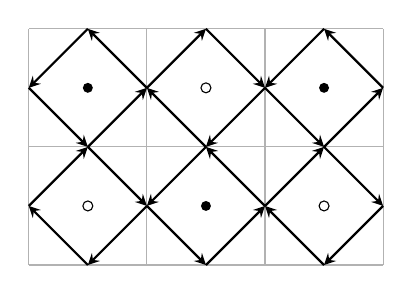
\begin{tikzpicture}[scale=1.5,>=stealth]
\draw[gray!60] (0,0) grid (3,2);
\foreach \i/\j in {1/1,3/1,2/2}{\draw (\i-0.5,\j-0.5) circle (1.2pt);
 \draw[->,thick] (\i-0.5,\j) -- (\i,\j-0.5); \draw[->,thick] (\i,\j-0.5) -- (\i-0.5,\j-1);
 \draw[->,thick] (\i-0.5,\j-1) -- (\i-1,\j-0.5); \draw[->,thick] (\i-1,\j-0.5) -- (\i-0.5,\j);}
\foreach \i/\j in {2/1,1/2,3/2}{\fill (\i-0.5,\j-0.5) circle (1.2pt);
 \draw[->,thick] (\i-0.5,\j) -- (\i-1,\j-0.5); \draw[->,thick] (\i-1,\j-0.5) -- (\i-0.5,\j-1);
 \draw[->,thick] (\i-0.5,\j-1) -- (\i,\j-0.5); \draw[->,thick] (\i,\j-0.5) -- (\i-0.5,\j);}
\end{tikzpicture}
\caption{The digraph $F'$ for $n=3$, $k=2$. White cells (hollow dots) are oriented clockwise, black cells
(solid dots) counter-clockwise.}\label{fig:Fprime}
\end{figure}

\begin{lemma}\label{lem:orient}
\textup{(i)} Every midpoint of a border side has exactly one arc of $F'$ entering and one leaving, and they are
the two arcs glued there. \textup{(ii)} Every midpoint $P$ of an internal side has exactly two arcs entering and
two leaving, one of each from either cell. If the side carries a mirror, each entering arc is glued to the
leaving arc of the same cell; if not, each entering arc is glued to the leaving arc of the other cell.
\end{lemma}

\begin{proof}
The arcs of a cell form a directed $4$-cycle through the four midpoints of its sides, so at each of these midpoints
one arc of the cell enters and one leaves. This proves (i) and the first sentence of (ii), and the statement about
mirrors, since a reflection glues the two arcs of the same cell.

Now let $P$ be the midpoint of an internal side $s$ without mirror, and suppose first that $s$ is vertical, with a
white cell $W$ on its left and a black cell $B$ on its right. The two arcs of $W$ at $P$ lie to the upper left and
lower left of $P$. Since $P$ is the rightmost point of the diamond of $W$ and this diamond is traversed clockwise,
it is traversed downwards at $P$: the upper-left arc enters $P$ and the lower-left arc leaves $P$. Likewise $P$ is
the leftmost point of the diamond of $B$, which is traversed counter-clockwise, hence also downwards at $P$: the
upper-right arc enters and the lower-right arc leaves. The collinear pairs are (upper left, lower right) and (upper
right, lower left), and each consists of an entering arc of one cell and a leaving arc of the other. If instead the
black cell is on the left, all four orientations are reversed and the same conclusion holds. The case of a
horizontal side follows by rotating the picture through $90^\circ$, which preserves the colouring pattern and the
sense of rotation.
\end{proof}

\begin{proposition}\label{prop:BEST}
$T(n,k)$ equals the number of Eulerian circuits of $F'$, and also the number $t_w(F')$ of spanning trees of $F'$
oriented towards any fixed vertex $w$.
\end{proposition}

\begin{proof}
By Lemma~\ref{lem:orient} the gluing at every vertex of $F'$ is a bijection between the entering and the leaving
arcs, so the mirror curve of $X$ is a decomposition of the arc set of $F'$ into directed closed trails. At a border
midpoint the bijection is forced; at an internal midpoint there are exactly two bijections between two entering
and two leaving arcs, and by Lemma~\ref{lem:orient}(ii) they correspond to ``mirror'' and ``no mirror''. Hence
mirror placements are in bijection with the systems of such bijections, and the mirror curve is a single polygon
exactly when the system is that of an Eulerian circuit (a closed trail through all arcs, considered up to cyclic
shifts). Every Eulerian circuit determines its system. So $T(n,k)$ is the number of Eulerian circuits of $F'$.

$F'$ is connected and every vertex has equal in- and out-degree, $1$ or $2$. By the BEST theorem
\cite{AEB,TS} the number of Eulerian circuits is $t_w(F')\prod_v(\dout(v)-1)!=t_w(F')$.
\end{proof}

\begin{remark}[Parity]\label{rem:parity}
Replacing the bijection at one internal midpoint by the other one either merges two closed trails or splits one,
so it changes the number of curves by exactly one. Since there are $\gcd(n,k)$ curves without mirrors
\cite{FM,Gerdes,JRSZ}, the number of curves of a placement $X$ is congruent to $\gcd(n,k)+|X|$ modulo $2$.
\end{remark}

We recall the matrix-tree theorem for digraphs \cite{Tutte}. For a finite digraph $D$ (loops and multiple arcs
allowed) with adjacency matrix $A$ and diagonal matrix $\Delta$ of out-degrees, put $L_D=\Delta-A$. For a vertex
$w$, the number $t_w(D)$ of spanning trees oriented towards $w$ (every vertex $v\ne w$ has exactly one arc of the
tree leaving it, and following these arcs leads to $w$) is the determinant of $L_D$ with row and column $w$
deleted.

\section{The corner digraph and line digraphs}\label{sec:line}

Call a corner $(p,q)$ \emph{even} or \emph{odd} according to the parity of $p+q$. Every side joins an even and an
odd corner. Let $\G=\G_{n,k}$ be the digraph on the $(n+1)(k+1)$ corners in which every vertical side is an arc
directed away from its even endpoint and every horizontal side is an arc directed away from its odd endpoint.
Thus each even corner sends an arc to each corner directly above or below it, each odd corner sends an arc to each
corner directly to its left or right, and every side is exactly one arc of $\G$.

Recall that the \emph{line digraph} $\mathcal L(D)$ of a digraph $D$ has the arcs of $D$ as vertices, with one arc
from $e$ to $e'$ whenever the head of $e$ is the tail of $e'$.

\begin{lemma}\label{lem:line}
Identifying each side with its midpoint, $F'=\mathcal L(\G)$.
\end{lemma}

\begin{proof}
Traverse the boundary of each white cell clockwise and of each black cell counter-clockwise. We claim that every
side of a cell is then traversed in its direction in $\G$. Consider the cell $Q_{ij}$. Its top side joins
$(i-1,j)$ and $(i,j)$. If $Q_{ij}$ is white, the side is traversed from $(i-1,j)$ to $(i,j)$, and its tail
$(i-1,j)$ is odd because $i+j$ is even; if $Q_{ij}$ is black it is traversed from $(i,j)$, which is then odd.
The right side joins $(i,j)$ and $(i,j-1)$: for a white cell it is traversed from $(i,j)$, which is even, and for
a black cell from $(i,j-1)$, which is even. The bottom and left sides are treated in the same way. This proves the
claim.

An arc of $F'$ in a cell $Q$ joins the midpoints of two consecutive sides $s,s'$ of $Q$ in the sense of traversal
of $Q$; by the claim the common corner of $s$ and $s'$ is the head of $s$ and the tail of $s'$ in $\G$. So every
arc of $F'$ is an arc of $\mathcal L(\G)$. Conversely, let the head of $s$ equal the tail of $s'$, say at the
corner $c$. If $c$ is even then $s'$ is vertical, and $s$, whose tail is odd, is horizontal; if $c$ is odd then
$s'$ is horizontal and $s$ is vertical. In both cases $s$ and $s'$ are perpendicular sides at $c$, hence two sides
of the cell $Q$ lying in the quadrant between them (which is one of the cells $Q_{ij}$, because $s$ and $s'$ lie in
the rectangle). By the claim, the traversal of $Q$ enters $c$ along $s$ and leaves along $s'$, so there is an arc of
$F'$ from $s$ to $s'$. Distinct arcs of $F'$ give distinct pairs $(s,s')$, and the correspondence is a bijection.
\end{proof}

The next lemma is due to Knuth \cite{Knuth} (see also \cite{Levine}); we include a short proof.

\begin{lemma}\label{lem:knuth}
Let $D$ be a finite digraph in which every vertex has out-degree at least $1$, and let $e_0$ be an arc from $u_0$ to
$v_0$. Then
\[ t_{e_0}\bigl(\mathcal L(D)\bigr)=\frac{t_{u_0}(D)}{\dout(v_0)}\prod_{v}\dout(v)^{\din(v)-1}. \]
\end{lemma}

\begin{proof}
Let $E$ and $V$ be the sets of arcs and vertices of $D$. Let $H$ and $R$ be the $E\times V$ matrices with
$H_{e,v}=1$ if $v$ is the head of $e$, $R_{e,v}=1$ if $v$ is the tail of $e$, and zero entries otherwise. Then
$HR^{\mathsf T}$ is the adjacency matrix of $\mathcal L(D)$ and $R^{\mathsf T}H$ is the adjacency matrix $A$ of
$D$. The out-degree of $e$ in $\mathcal L(D)$ is $\dout(\mathrm{head}(e))$; let $\Delta'$ be the corresponding
diagonal $E\times E$ matrix and $\Delta$ the diagonal matrix of out-degrees of $D$, so that $\Delta'H=H\Delta$.

Denote by $H_0,R_0,\Delta'_0$ the matrices obtained by deleting the row (and for $\Delta'$ also the column) of
$e_0$. By the matrix-tree theorem and the identity $\det(I-PQ)=\det(I-QP)$,
\[
t_{e_0}(\mathcal L(D))=\det\bigl(\Delta'_0-H_0R_0^{\mathsf T}\bigr)
=\det(\Delta'_0)\,\det\bigl(I_V-R_0^{\mathsf T}(\Delta'_0)^{-1}H_0\bigr).
\]
The $(c,c')$ entry of $R_0^{\mathsf T}(\Delta'_0)^{-1}H_0$ is the number of arcs $e\neq e_0$ from $c$ to $c'$ divided
by $\dout(c')$, so $R_0^{\mathsf T}(\Delta'_0)^{-1}H_0=(A-E_{u_0v_0})\Delta^{-1}$, where $E_{u_0v_0}$ is a matrix
unit. Moreover $\det\Delta'_0=\prod_{v}\dout(v)^{\din(v)}/\dout(v_0)$. Therefore
\[
t_{e_0}(\mathcal L(D))=\frac{1}{\dout(v_0)}\prod_v\dout(v)^{\din(v)-1}\cdot\det\bigl(L_D+E_{u_0v_0}\bigr).
\]
Expanding along row $u_0$, $\det(L_D+E_{u_0v_0})=\det L_D+C_{u_0v_0}=C_{u_0v_0}$, the $(u_0,v_0)$ cofactor of
$L_D$, since $L_D$ has zero row sums. Finally, the cofactors of $L_D$ that lie in the same row are all equal: from $L_D\,\mathrm{adj}(L_D)=0$, every
column of $\mathrm{adj}(L_D)$ lies in the kernel of $L_D$, which is spanned by the all-ones vector if $L_D$ has
corank $1$, while $\mathrm{adj}(L_D)=0$ if the corank is larger. Hence $C_{u_0v_0}=C_{u_0u_0}=t_{u_0}(D)$.
\end{proof}

\begin{proposition}\label{prop:gamma}
For every arc of $\G$ from $u_0$ to $v_0$,
\[ T(n,k)=\frac{2^{(n-1)(k-1)}\;t_{u_0}(\G)}{\dout(v_0)}. \]
\end{proposition}

\begin{proof}
By Proposition~\ref{prop:BEST}, Lemma~\ref{lem:line} and Lemma~\ref{lem:knuth} it suffices to show that
$\prod_c\dout(c)^{\din(c)-1}=2^{g}$. Each of the $g$ interior corners has two horizontal and two vertical sides,
hence $\dout=\din=2$. A boundary corner that is not one of the four extreme corners has three sides, two along the
boundary and one perpendicular to it; so either $\dout=2$ and $\din=1$, or $\dout=1$ and $\din=2$. The four
extreme corners have $\dout=\din=1$. In all boundary cases $(\dout)^{\din-1}=1$.
\end{proof}

Taking $u_0=(1,0)$ and $v_0=(0,0)$, for which $\dout(v_0)=1$, gives Corollary~\ref{cor:div}.

\section{Counting the trees of $\G$}\label{sec:eval}

Write $\dhh(p)=1$ if $p\in\{0,n\}$ and $\dhh(p)=2$ otherwise, and $\dvv(q)=1$ if $q\in\{0,k\}$ and $\dvv(q)=2$
otherwise; these are the numbers of horizontal, respectively vertical, sides at a corner $(p,q)$. So
$\dout(p,q)=\dvv(q)$ for even corners and $\dout(p,q)=\dhh(p)$ for odd corners. Let $\mathcal E$ and $\mathcal O$
be the sets of even and odd corners. Since the arcs of $\G$ are the sides,
\begin{equation}\label{eq:outprod}
\sum_c\dout(c)=2nk+n+k,\qquad\text{hence}\qquad \prod_c\dout(c)=2^{\,2nk+n+k-(n+1)(k+1)}=2^{\,nk-1},
\end{equation}
because every out-degree is $1$ or $2$.

Fix an odd corner $u_0$. With rows and columns ordered as $(\mathcal E,\mathcal O)$,
\[ L_{\G}=\begin{pmatrix} D_{\mathcal E} & -B\\ -C & D_{\mathcal O}\end{pmatrix}, \]
where $D_{\mathcal E}=\mathrm{diag}(\dvv(q))$, $D_{\mathcal O}=\mathrm{diag}(\dhh(p))$, $B_{e,o}=1$ if $o$ is
directly above or below $e$, and $C_{o,e}=1$ if $e$ is directly left or right of $o$. Deleting the row and
column of $u_0$ and taking the Schur complement of the block $D_{\mathcal E}$,
\begin{equation}\label{eq:schur}
t_{u_0}(\G)=\det(D_{\mathcal E})\cdot\det\bigl(S^{(u_0)}\bigr),\qquad S=D_{\mathcal O}-C\,D_{\mathcal E}^{-1}B,
\end{equation}
where $S^{(u_0)}$ is $S$ with row and column $u_0$ deleted. Put $\Xi=D_{\mathcal O}^{-1}S$, an
$\mathcal O\times\mathcal O$ matrix; then
\begin{equation}\label{eq:xi}
\det\bigl(S^{(u_0)}\bigr)=\frac{\prod_{o\in\mathcal O}\dhh(p_o)}{\dhh(p_{u_0})}\,\det\bigl(\Xi^{(u_0)}\bigr).
\end{equation}

\begin{lemma}\label{lem:spec}
Let $\lambda_{l,m}=1-\cos\frac{l\pi}{n}\cos\frac{m\pi}{k}$ for $0\le l\le n$, $0\le m\le k$, and let $\iota$ be
the involution $(l,m)\mapsto(n-l,k-m)$ of the index set. Then $\Xi$ is diagonalisable, and its eigenvalues, with
multiplicity, are the numbers $\lambda_{l,m}$, one for each two-element orbit of $\iota$.
\textup{(}Note $\lambda_{\iota(l,m)}=\lambda_{l,m}$.\textup{)}
\end{lemma}

\begin{proof}
Let $\mathcal K$ be the operator on real functions on the set of all corners given by
\[ (\mathcal Kf)(p,q)=\dhh(p)f(p,q)-\sum_{p'=p\pm1}\ \frac{1}{\dvv(q)}\sum_{q'=q\pm1}f(p',q'), \]
where the sums run over those values for which $(p',q)$, respectively $(p',q')$, is a corner. $\mathcal K$ maps
functions supported on $\mathcal O$ to functions supported on $\mathcal O$, and on these it acts as the matrix
$S$: the inner average is $D_{\mathcal E}^{-1}B$ and the outer sum is $C$.

Let $\varphi_l(p)=\cos(l\pi p/n)$ and $\psi_m(q)=\cos(m\pi q/k)$. For $0<p<n$ we have
$\varphi_l(p-1)+\varphi_l(p+1)=2\cos\frac{l\pi}n\,\varphi_l(p)$, while
$\varphi_l(1)=\cos\frac{l\pi}n\,\varphi_l(0)$ and $\varphi_l(n-1)=\cos\frac{l\pi}n\,\varphi_l(n)$; in all cases
$\sum_{p'=p\pm1}\varphi_l(p')=\dhh(p)\cos\frac{l\pi}n\varphi_l(p)$. In the same way
$\dvv(q)^{-1}\sum_{q'=q\pm1}\psi_m(q')=\cos\frac{m\pi}{k}\psi_m(q)$. Hence
\[ \mathcal K(\varphi_l\otimes\psi_m)=\lambda_{l,m}\,\dhh\cdot(\varphi_l\otimes\psi_m), \]
where $(\varphi\otimes\psi)(p,q)=\varphi(p)\psi(q)$. The vectors $\varphi_0,\dots,\varphi_n$ are eigenvectors of
the matrix $\bigl(\dhh(p)^{-1}[\,|p-p'|=1\,]\bigr)$ for the $n+1$ distinct eigenvalues $\cos(l\pi/n)$, so they form
a basis of $\mathbb R^{n+1}$; similarly for the $\psi_m$. Thus the $(n+1)(k+1)$ functions
$\varphi_l\otimes\psi_m$ form a basis of the space of all functions on the corners.

Since $\varphi_{n-l}(p)=(-1)^p\varphi_l(p)$ and $\psi_{k-m}(q)=(-1)^q\psi_m(q)$, the function
\[ h_{l,m}=\varphi_l\otimes\psi_m-\varphi_{n-l}\otimes\psi_{k-m}=\bigl(1-(-1)^{p+q}\bigr)\varphi_l\otimes\psi_m \]
is supported on $\mathcal O$, and it satisfies $\mathcal K h_{l,m}=\lambda_{l,m}\,\dhh\, h_{l,m}$, that is,
$\Xi h_{l,m}=\lambda_{l,m}h_{l,m}$. Choosing one $(l,m)$ from each two-element orbit of $\iota$ gives linearly
independent functions $h_{l,m}$. Their number is $\tfrac12\bigl((n+1)(k+1)-\epsilon\bigr)$, where $\epsilon=1$ if
$n$ and $k$ are both even ($\iota$ then has the single fixed point $(n/2,k/2)$) and $\epsilon=0$ otherwise. This is
exactly $|\mathcal O|$. So the $h_{l,m}$ form a basis of eigenvectors of $\Xi$.
\end{proof}

The eigenvalue $\lambda_{l,m}$ vanishes only for $(l,m)\in\{(0,0),(n,k)\}$, a single orbit; so $0$ is a simple
eigenvalue of $\Xi$. Let $\Pi'$ denote the product of the nonzero eigenvalues of $\Xi$.

\begin{lemma}\label{lem:adj}
For every odd corner $u_0=(p_0,q_0)$,
\[ \det\bigl(\Xi^{(u_0)}\bigr)=\Pi'\cdot\frac{\dhh(p_0)\,\dvv(q_0)}{2nk}. \]
\end{lemma}

\begin{proof}
Let $X$ be a square matrix with a simple eigenvalue $0$, with $Xr=0$ and $\ell^{\mathsf T}X=0$ for nonzero vectors
$r,\ell$. Then $X$ has corank $1$, its adjugate satisfies $X\,\mathrm{adj}(X)=\mathrm{adj}(X)\,X=0$ and so
$\mathrm{adj}(X)=\alpha\,r\ell^{\mathsf T}$ for a scalar $\alpha$; its trace is the sum of the principal minors
of corank one, which equals the product $\Pi'$ of the nonzero eigenvalues. Hence
$\alpha\,\ell^{\mathsf T}r=\Pi'$, and the principal minor obtained by deleting row and column $u$ is
$\Pi'\,r_u\ell_u/(\ell^{\mathsf T}r)$.

For $X=\Xi$ we may take $r=\mathbf 1$, because $L_\G$ has zero row sums, i.e.\ $B\mathbf 1=D_{\mathcal E}\mathbf 1$
and $C\mathbf 1=D_{\mathcal O}\mathbf 1$, whence $S\mathbf 1=0$. We claim that $\ell(p,q)=\dhh(p)\dvv(q)$ works.
Indeed $\ell^{\mathsf T}\Xi=y^{\mathsf T}S$ with $y(p,q)=\dvv(q)$. For an even corner $e=(p,q)$,
$(y^{\mathsf T}C)_e=\dhh(p)\dvv(q)$, since $e$ has $\dhh(p)$ horizontal neighbours, all in row $q$; hence
$(y^{\mathsf T}CD_{\mathcal E}^{-1})_e=\dhh(p)$, and for an odd corner $o=(p,q)$,
$(y^{\mathsf T}CD_{\mathcal E}^{-1}B)_o=\dvv(q)\dhh(p)=(y^{\mathsf T}D_{\mathcal O})_o$. So $y^{\mathsf T}S=0$.

It remains to compute $\ell^{\mathsf T}r$, the sum of $\dhh(p)\dvv(q)$ over the odd corners. The sum over all
corners is $\sum_p\dhh(p)\sum_q\dvv(q)=2n\cdot 2k$, and the signed sum
\[ \sum_{(p,q)}(-1)^{p+q}\dhh(p)\dvv(q)=\Bigl(\sum_{p=0}^{n}(-1)^p\dhh(p)\Bigr)\Bigl(\sum_{q=0}^{k}(-1)^q\dvv(q)\Bigr) \]
vanishes because $\sum_{p=0}^{n}(-1)^p\dhh(p)=0$. Hence $\ell^{\mathsf T}r=2nk$.
\end{proof}

\begin{lemma}\label{lem:trig}
$\displaystyle \Pi'=\frac{nk}{2^{\,n+k-3}}\ \prod_{l=1}^{n-1}\prod_{m=1}^{k-1}\lambda_{l,m}^{1/2}$.
\end{lemma}

\begin{proof}
All $\lambda_{l,m}$ are nonnegative, and if $\iota$ has a fixed point $(n/2,k/2)$ then
$\lambda_{n/2,k/2}=1$. By Lemma~\ref{lem:spec}, $(\Pi')^2$ is therefore the product of $\lambda_{l,m}$ over
all $(l,m)\notin\{(0,0),(n,k)\}$. Split this index set into the interior $0<l<n$, $0<m<k$, the column $l=0$
($1\le m\le k$), the column $l=n$ ($0\le m\le k-1$), and the rows $m=0$ and $m=k$ ($0<l<n$). Using
$\prod_{j=1}^{N-1}2\sin\frac{j\pi}{N}=N$ with $N=2n$ one finds $\prod_{l=1}^{n-1}2\sin\frac{l\pi}{2n}=\sqrt n$,
and therefore
\[ \prod_{l=1}^{n-1}\Bigl(1-\cos\frac{l\pi}n\Bigr)=\prod_{l=1}^{n-1}2\sin^2\frac{l\pi}{2n}=\frac{n}{2^{n-1}}
=\prod_{l=1}^{n-1}\Bigl(1+\cos\frac{l\pi}n\Bigr). \]
So each of the rows $m=0$ and $m=k$ contributes $n/2^{n-1}$, and each of the columns $l=0$ and $l=n$ contributes
$2\cdot k/2^{k-1}$ (the extra factor $2$ is $\lambda_{0,k}=\lambda_{n,0}=2$). The product of the four boundary
contributions is $\bigl(nk/2^{\,n+k-3}\bigr)^2$.
\end{proof}

\begin{proof}[Proof of Theorem~\ref{thm:main}]
Let $u_0=(p_0,q_0)$ be an odd corner and $v_0$ a corner directly left or right of it; then $v_0$ is even and
$\dout(v_0)=\dvv(q_0)$. By \eqref{eq:schur}, \eqref{eq:xi}, Lemma~\ref{lem:adj} and \eqref{eq:outprod},
\[
t_{u_0}(\G)=\prod_{e\in\mathcal E}\dvv(q_e)\prod_{o\in\mathcal O}\dhh(p_o)\cdot\frac{\dvv(q_0)\,\Pi'}{2nk}
=2^{\,nk-1}\cdot\frac{\dvv(q_0)\,\Pi'}{2nk}.
\]
Proposition~\ref{prop:gamma} and Lemma~\ref{lem:trig} now give
\[
T(n,k)=2^{\,g}\cdot 2^{\,nk-1}\cdot\frac{1}{2nk}\cdot\frac{nk}{2^{\,n+k-3}}\prod_{l=1}^{n-1}\prod_{m=1}^{k-1}\lambda_{l,m}^{1/2}
=2^{\,g+nk-n-k+1}\prod_{l,m}\lambda_{l,m}^{1/2},
\]
and $g+nk-n-k+1=2g$. This is \eqref{eq:main}.
\end{proof}

\section{Proofs of the corollaries}

\begin{proof}[Proof of Corollary~\ref{cor:rows}]
Write $c_l=\cos\frac{l\pi}{n}$, $c'_m=\cos\frac{m\pi}{k}$, and distribute the prefactor of \eqref{eq:main} as
$4^{(n-1)(k-1)}=\prod_{l=1}^{n-1}4^{k-1}$. If $n$ is even, the factors with $l=n/2$ are all equal to $1$, and
this index contributes its share $4^{k-1}=\varepsilon_n^{\,k-1}$.
For $l<n/2$, the factors with indices $l$ and $n-l$, together with their share $16^{k-1}$, contribute
\[ 16^{k-1}\prod_{m=1}^{k-1}\bigl(1-c_lc'_m\bigr)^{1/2}\bigl(1+c_lc'_m\bigr)^{1/2}
=\prod_{m=1}^{k-1}\bigl(16-16\,c_lc'_m\bigr), \]
because $\prod_m(1+c_lc'_m)=\prod_m(1-c_lc'_{k-m})=\prod_m(1-c_lc'_m)$. Recall that the Chebyshev polynomial
of the second kind satisfies
\[ U_{k-1}(x)=\prod_{m=1}^{k-1}\Bigl(2x-2\cos\frac{m\pi}{k}\Bigr),\qquad U_{k}=2xU_{k-1}-U_{k-2},\quad U_{-1}=0,\ U_0=1. \]
So the product above equals $(8c_l)^{k-1}U_{k-1}(1/c_l)$, and the recurrence for $U_k$ shows that it is
$F_{n,l}(k)$.

(a) For $n=2$ the product is empty. (b) For $n=3$, $c_1^2=\frac14$, so $F(k+1)=16F(k)-16F(k-1)$ and
$F(k)=4^{k-1}a(k)$. (c) For $n=4$, $c_1^2=\frac12$ and $T(4,k)=4^{k-1}F_{4,1}(k)$ with
$F(k+1)=16F(k)-32F(k-1)$; multiplying by $4^{k}$ gives the recurrence, valid for $k\ge3$ (and for $k=2$ with
$T(4,0)=0$).

For (d) and (e) we use the following fact. If $x^2-P_1x+Q_1$ has distinct roots and annihilates the sequence $a$,
and $x^2-P_2x+Q_2$ has distinct roots and annihilates $b$, then $a(k)b(k)$ is a combination of the $k$-th powers of
the four products of a root of the first with a root of the second polynomial, and is therefore annihilated by
\[ x^4-P_1P_2\,x^3+\bigl(P_1^2Q_2+P_2^2Q_1-2Q_1Q_2\bigr)x^2-P_1P_2Q_1Q_2\,x+Q_1^2Q_2^2 . \]
Here $P_1=P_2=16$ and $Q_i=64c_i^2$, with roots $8\pm8\sin\frac{i\pi}{n}$. For $n=5$:
$c_1^2=\frac{3+\sqrt5}{8}$, $c_2^2=\frac{3-\sqrt5}{8}$, so $Q_1+Q_2=48$, $Q_1Q_2=256$ and the polynomial is
$x^4-256x^3+11776x^2-65536x+65536$. For $n=6$: $c_1^2=\frac34$, $c_2^2=\frac14$, so $Q_1=48$, $Q_2=16$ and
$F_{6,1}F_{6,2}$ is annihilated by $x^4-256x^3+14848x^2-196608x+589824$; multiplying the sequence by $4^{k-1}$
multiplies the roots by $4$ and gives $x^4-1024x^3+237568x^2-12582912x+150994944$. The recurrences hold for all
$k$ for which the indices are at least $0$, in particular for $k\ge5$.
\end{proof}

\begin{proof}[Proof of Corollary~\ref{cor:ineq}]
In \eqref{eq:main2} every factor lies in $(0,1]$. A factor equals $1$ only if one of the two cosines
vanishes, which does not happen for $1\le l<n/2$ and $1\le m<k/2$. The product is empty exactly when $n\le2$ or
$k\le2$.
\end{proof}

\begin{proof}[Proof of Corollary~\ref{cor:growth}]
By \eqref{eq:main2}, $\log T(n,k)=2(n-1)(k-1)\log 2+\sum f\bigl(\frac{l\pi}{n},\frac{m\pi}{k}\bigr)$, summed over
$1\le l<n/2$, $1\le m<k/2$, where $f(x,y)=\log(1-\cos^2x\cos^2y)$. On $(0,\frac\pi2]^2$ the function $f$ is
nonpositive, nondecreasing in each variable, and integrable (near the origin $1-\cos^2x\cos^2y\ge c\,(x^2+y^2)$ for
some $c>0$). By monotonicity each term, multiplied by the mesh area $\frac{\pi^2}{nk}$, lies between the integrals of
$f$ over the mesh cell to its lower left and over the mesh cell to its upper right (where $f$ is continued by $0$
outside $(0,\frac\pi2]^2$), so $\frac{\pi^2}{nk}\sum f\to\int_0^{\pi/2}\!\!\int_0^{\pi/2}f$. By the symmetries
$x\mapsto\pi-x$, $y\mapsto\pi-y$ this integral equals $\frac{\pi^2}{2}I$ with
$I=\pi^{-2}\int_0^\pi\!\!\int_0^\pi\log(1-\cos x\cos y)\,dx\,dy$. Using
$\frac1\pi\int_0^\pi\log(1-a\cos x)\,dx=\log\frac{1+\sqrt{1-a^2}}{2}$ for $|a|\le1$ and
$\int_0^{\pi}\log(1+\sin y)\,dy=4G-\pi\log2$ we get $I=\frac{4G}{\pi}-2\log 2$, and the limit of $\frac{1}{nk}\log T(n,k)$ is
$2\log2+\frac12 I=\log 2+\frac{2G}{\pi}$.
\end{proof}

\section{Remarks}

\begin{remark}[Manhattan lattice]\label{rem:manhattan}
In the coordinates $(x+y,x-y)$ the digraph $F'$ is a square lattice in which all arcs on a line point the same way
and adjacent parallel lines point in opposite ways, that is, a piece of the Manhattan lattice with reflecting
boundary. If each internal side receives a mirror independently with probability $\frac12$, then $T(n,k)/2^{M}$ is
the probability that all trajectories form a single loop; random mirrors on the infinite Manhattan lattice have
been studied in physics in connection with localisation \cite{BOC}. The digraph $\G$, in which a walker must turn
at every corner, is known as the L-lattice; that the Manhattan lattice is its line digraph (``covering lattice'')
goes back to Kasteleyn \cite{Kasteleyn}. A Hamiltonian circuit of a line digraph $\mathcal L(D)$ is an Eulerian
circuit of $D$, so the Hamiltonian walks on the Manhattan lattice counted in \cite{Kasteleyn} are Eulerian circuits
of the L-lattice, whereas $T(n,k)$ counts Eulerian circuits of the Manhattan lattice itself. Hamiltonian walks on
Manhattan lattices with rectangular and other boundaries are studied in \cite{DD}.
\end{remark}

\begin{remark}[Spanning trees]\label{rem:trees}
By Theorem~\ref{thm:main}, $T(n,k)^2=4^{(n-1)(k-1)}\det\bigl(4I-A_{n-1}\otimes A_{k-1}\bigr)$. The matrix
$4I-A_{n-1}\otimes A_{k-1}$ is indexed by the interior corners; its off-diagonal entries are $-1$ for pairs of
diagonally adjacent corners. Let $D$ be the graph whose vertices are the interior corners and one further vertex
$b$, with an edge between any two diagonally adjacent interior corners and, for every interior corner, one edge to
$b$ for each of its four diagonal neighbours that lies on the boundary. The matrix above is the Laplacian of $D$
with the row and column of $b$ deleted, so by the matrix-tree theorem $T(n,k)^2$ is $4^{(n-1)(k-1)}$ times the
number of spanning trees of $D$.
\end{remark}

\begin{remark}[Other shapes]\label{rem:shapes}
Lemma~\ref{lem:orient} and Proposition~\ref{prop:BEST} use only the chessboard colouring and not the rectangular
shape. For every finite set of cells, the number of mirror placements with a single curve equals the number of
spanning trees of the corresponding digraph $F'$ oriented towards a fixed vertex, which is a determinant. For the
diamond-shaped arrays with rows of $1,3,\dots,2r-1,\dots,3,1$ dots this gives
\[ 1,\quad 1,\quad 240,\quad 11\,661\,312,\quad 99\,623\,930\,691\,584,\quad
144\,999\,115\,803\,453\,250\,600\,960 \]
for $r=1,\dots,6$;
the values for $r=3,4$ agree with the exhaustive counts of \cite{YN}. Lemma~\ref{lem:line} fails for every shape with a
re-entrant corner, where two perpendicular sides meet without a cell between them, and we do not know a product
formula for the diamonds.
\end{remark}

\begin{remark}[Computations]\label{rem:comp}
\emergencystretch=1.5em
The following was checked by computer; the programs are available at
\url{https://github.com/cyrilshtabtsovsky/light-in-a-box-of-mirrors} and are archived with this paper at \url{https://doi.org/10.5281/zenodo.24546586}.
A direct simulation of the definition agrees with \eqref{eq:main} for all grids with at most $27$ internal sides,
the largest being $2\times9$, $3\times6$ and $4\times4$. Formula \eqref{eq:main}, evaluated exactly through the
determinant in Theorem~\ref{thm:main}, agrees with all $136$ terms listed in \cite{OEIS} ($n+k\le17$).
The tree counts of Propositions~\ref{prop:BEST} and~\ref{prop:gamma} were computed in exact arithmetic for
$n,k\le 8$ and agree with \eqref{eq:main}. Lemma~\ref{lem:line} was checked for $n,k\le6$, Lemmas~\ref{lem:spec}
and~\ref{lem:adj} in floating-point arithmetic for $n,k\le6$, and items (c)--(e) of Corollary~\ref{cor:rows} for
$k\le40$. Remark~\ref{rem:parity} was checked for all placements on the grids with at most $12$ internal sides and for random
placements with $n,k\le6$, Remark~\ref{rem:trees} for $n,k\le7$, and
the determinant of Remark~\ref{rem:shapes} against a direct simulation for $r\le3$ and for three non-rectangular
shapes.
\end{remark}

\section*{Statement on the use of AI}
This work was carried out with the AI system Claude (Anthropic), model Claude Fable~5.2 at the high effort
setting, in one working session on 25--26 November 2026. The problem was selected by the author from a list of
open problems compiled with Claude in the same session. The model found formula \eqref{eq:main} and the proof, wrote the programs of
Remark~\ref{rem:comp}, carried out the literature search, and wrote the text, which was revised at the author's
direction. The proof has been tested by the computations of Remark~\ref{rem:comp}; it has not been formalised in
a proof assistant. The author takes responsibility for the content.

\begin{thebibliography}{99}
\bibitem{AEB} T.~van Aardenne-Ehrenfest and N.~G.~de Bruijn, Circuits and trees in oriented linear graphs,
\emph{Simon Stevin} \textbf{28} (1951), 203--217.
\bibitem{BOC} E.~J.~Beamond, A.~L.~Owczarek and J.~Cardy, Quantum and classical localisation and the Manhattan
lattice, arXiv:cond-mat/0210359, 2002.
\bibitem{DD} B.~Duplantier and F.~David, Exact partition functions and correlation functions of multiple
Hamiltonian walks on the Manhattan lattice, \emph{J. Stat. Phys.} \textbf{51} (1988), 327--434.
\bibitem{FM} G.~Fisher and B.~Mellor, On the topology of Celtic knot designs, in \emph{Bridges: Mathematical
Connections in Art, Music, and Science} (2004), 37--44.
\bibitem{Gerdes} P.~Gerdes, \emph{Geometry from Africa: Mathematical and Educational Explorations}, Mathematical
Association of America, 1999.
\bibitem{Ishimoto} Y.~Ishimoto, Solving infinite kolam in knot theory, arXiv:0710.1976, 2007.
\bibitem{JRSZ} S.~Jablan, L.~Radovi\'c, R.~Sazdanovi\'c and A.~Zekovi\'c, Mirror-curves and knot mosaics,
arXiv:1106.3784, 2011.
\bibitem{Kasteleyn61} P.~W.~Kasteleyn, The statistics of dimers on a lattice. I. The number of dimer arrangements
on a quadratic lattice, \emph{Physica} \textbf{27} (1961), 1209--1225.
\bibitem{Kasteleyn} P.~W.~Kasteleyn, A soluble self-avoiding walk problem, \emph{Physica} \textbf{29} (1963),
1329--1337.
\bibitem{KPW} R.~W.~Kenyon, J.~G.~Propp and D.~B.~Wilson, Trees and matchings, \emph{Electron. J. Combin.}
\textbf{7} (2000), Research Paper~25.
\bibitem{Knuth} D.~E.~Knuth, Oriented subtrees of an arc digraph, \emph{J. Combinatorial Theory} \textbf{3} (1967),
309--314.
\bibitem{Levine} L.~Levine, Sandpile groups and spanning trees of directed line graphs, \emph{J. Combin. Theory
Ser.~A} \textbf{118} (2011), 350--364.
\bibitem{Nagata} S.~Nagata, How many loops Kolam loop pattern consists of, \emph{Forma} \textbf{30} (2015), 9--18.
\bibitem{OEIS} K.~Sharma, Sequence A400778, in \emph{The On-Line Encyclopedia of Integer Sequences},
\url{https://oeis.org/A400778}, November 2026.
\bibitem{TF} H.~N.~V.~Temperley and M.~E.~Fisher, Dimer problem in statistical mechanics---an exact result,
\emph{Philos. Mag.} \textbf{6} (1961), 1061--1063.
\bibitem{TS} W.~T.~Tutte and C.~A.~B.~Smith, On unicursal paths in a network of degree 4, \emph{Amer. Math. Monthly}
\textbf{48} (1941), 233--237.
\bibitem{Tutte} W.~T.~Tutte, The dissection of equilateral triangles into equilateral triangles, \emph{Proc.
Cambridge Philos. Soc.} \textbf{44} (1948), 463--482.
\bibitem{YN} K.~Yanagisawa and S.~Nagata, Fundamental study on design system of Kolam pattern, \emph{Forma}
\textbf{22} (2007), 31--46.
\end{thebibliography}

\end{document}
